\documentclass[tikz,border=3mm,multi=tikzpicture]{standalone}
\usepackage[utf8]{inputenc}
\usepackage[T1]{fontenc}
\usepackage{helvet}
\renewcommand{\familydefault}{\sfdefault}
\usepackage{tikz}
\usetikzlibrary{arrows.meta,positioning,calc}
\begin{document}

\tikzset{every node/.append style={font=\sffamily\small}}
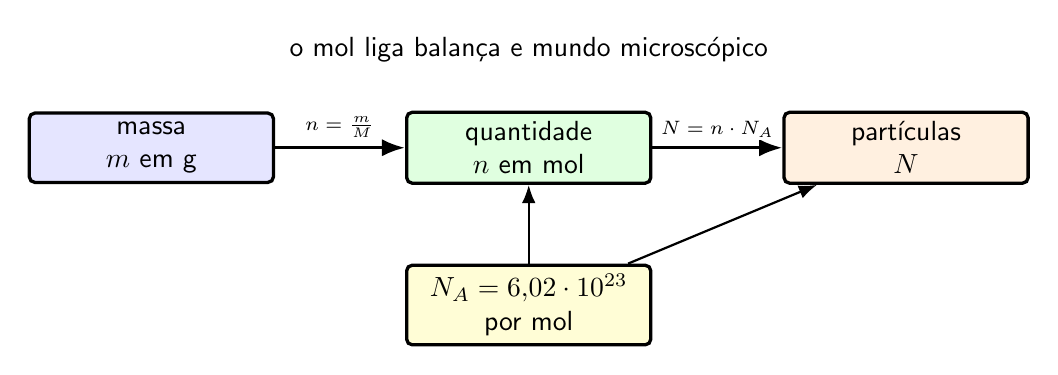
\begin{tikzpicture}[>=Latex,node distance=0.9cm]
  \tikzstyle{box}=[draw,rounded corners=2pt,very thick,minimum width=3.1cm,minimum height=0.85cm,align=center]
  \node[box,fill=blue!10] (massa) {massa\\$m$ em g};
  \node[box,fill=green!12,right=1.65cm of massa] (mol) {quantidade\\$n$ em mol};
  \node[box,fill=orange!12,right=1.65cm of mol] (part) {partículas\\$N$};
  \draw[very thick,->] (massa) -- (mol) node[midway,above=0.08cm,fill=white,inner sep=1pt,font=\sffamily\scriptsize] {$n=\frac{m}{M}$};
  \draw[very thick,->] (mol) -- (part) node[midway,above=0.08cm,fill=white,inner sep=1pt,font=\sffamily\scriptsize] {$N=n\cdot N_A$};
  \node[box,fill=yellow!16,below=1.0cm of mol] (na) {$N_A=6{,}02\cdot10^{23}$\\por mol};
  \draw[thick,->] (na) -- (mol);
  \draw[thick,->] (na) -- (part);
  \node[align=center,above=0.5cm of mol] {o mol liga balança e mundo microscópico};
\end{tikzpicture}

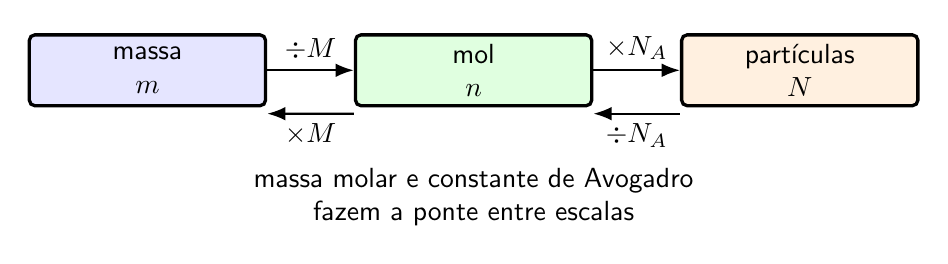
\begin{tikzpicture}[>=Latex,node distance=1.0cm]
  \tikzstyle{box}=[draw,rounded corners=2pt,very thick,minimum width=3.0cm,minimum height=0.9cm,align=center]
  \node[box,fill=blue!10] (massa) {massa\\$m$};
  \node[box,fill=green!12,right=1.1cm of massa] (mol) {mol\\$n$};
  \node[box,fill=orange!12,right=1.1cm of mol] (part) {partículas\\$N$};
  \draw[->,thick] (massa) -- node[above] {$\div M$} (mol);
  \draw[->,thick] ($(mol.south west)+(0,-0.08)$) -- node[below] {$\times M$} ($(massa.south east)+(0,-0.08)$);
  \draw[->,thick] (mol) -- node[above] {$\times N_A$} (part);
  \draw[->,thick] ($(part.south west)+(0,-0.08)$) -- node[below] {$\div N_A$} ($(mol.south east)+(0,-0.08)$);
  \node[align=center,below=0.65cm of mol] {massa molar e constante de Avogadro\\fazem a ponte entre escalas};
\end{tikzpicture}
\end{document}
